\section*{Sudoku Löser basierend auf einem genetischen Algorithmus}
Ziel dieses Projektes ist es Sudoku beliebiger Form mithilfe von genetischen Algorithmen zu lösen.
Das bedeutet die Felder eines vorgegebenen Sudokus so auszufüllen, dass in keiner Reihe, Spalte und keinem Block Zahlen doppelt vorkommen. 
Im Datensatz der hier zu lösenden Sudokus befinden sich hauptsächlich 9x9 Sudokus, aber auch wenige 25x25 Sudokus (Code/data.zip).

\subsection*{Erklärung der Bestandteile}
\subsubsection*{1. Sudoku-Representation}

In Sudoku.hpp (Code/Sudoku.hpp) wird die Klasse Sudoku definiert. Diese enthält neben Daten zur Gesamtgröße auch öfter verwendete Teilgrößen wie die Größe eines Blocks oder die Anzahl der Blöcke. Die Zahlen des Sudokus sind für einfacheren Zugriff in 2 verschiedenen Datenstrukturen gespeichert, die beide Zugriff auf 
die gleichen shared\_ptr haben. Dabei ist die row\_representation ein fortgehender 1D-Vektor, der die Reihen hintereinander speichert. Die grid\_representation
ist ein 2D-Vektor, der in der ersten Dimension die Blöcke und in der zweiten Dimension die Reihen innerhalb der Blöcke speichert. Neben dem Standardkonstruktor werden auch ein Copy-Konstruktor, welcher eine tiefe Kopie erstellt und ein Size-Konstruktor, welcher ein mit Nullen gefülltes Sudoku der gegebenen Größe erstellt, implementiert. Bei jedem Konstruktor wird automatisch auch die grid\_representation erstellt.
Es stehen außerdem Getter-,Setter- sowie Ausgabefunktionen bereit.

\noindent Weiterhin ist die Klasse generisch implementiert, sodass sowohl float, als auch int Datentypen verwendet werden können. Die float Variante ist für das Berechnen von individuellen Fitnessbewertungen wichtig.

\subsubsection*{2. Generation und Operatoren}

In Generation.hpp (Code/Generation.hpp) werden alle anderen wichtigen Funktionalitäten definiert. In dieser werden die ursprüngliche Populationsgröße und die momentan vorhandene gespeichert. Die Klasse hat neben dem original Sudoku, also dem ursprünglich gegebenem Input mit leeren Feldern, auch eine Menge von Lösungskandidaten (population). Für die Fitness werden außerdem die Fitnesswerte der gesamten Sudokus (fitness\_sums), aber auch die der individuellen Felder (fitness\_sudokus) gespeichert. Neben dem default Konstruktor existiert ein Konstruktor, der aus einem gegebenen Sudoku und einer Populationsgröße eine Population erstellt und diese je nach gewählter Methode initialisiert.

\noindent\textbf{2.1. Initialisierung}

\noindent Für die Initialisierung können 2 verschiedene Methoden verwendet werden. Beide iterieren über jedes Element der Population.
\begin{enumerate}
    \item Zufällige Initialisierung: Jedem Feld wird eine zufällige Zahl zugeordnet (1-9). Dabei wird allerdings darauf geachtet, dass in keinem Block eine Zahl doppelt vorkommt.
    \item Schlaue Initialisierung: ist eine Erweiterung, die bei der Initialisierung nicht nur auf keine Kollisionen im Block achtet, sondern dazu auch zufällig
    horizontal oder vertikal wählt und auch dort versucht die Kollisionen mit Reihen bzw. Spalten zu vermeiden. Das ist natürlich nicht immer mit wenig Rechenaufwand möglich.
    Daher werden die wenigen Felder, für die sich keine Kandidaten in linearer Laufzeit findet, der nicht mit Reihe bzw. Spalte kollidiert, zufällig so belegt, dass wenigstens die Kollision im Block verhindert wird.
\end{enumerate}

\noindent\textbf{2.2 Crossover}

\noindent Für die Crossover Operation wird eine Operation definiert, die einen Wert n bekommt. Getauscht werden die n-1 Reihen von Blöcken jedes Elternteils mit n-1 Reihen des anderen. Wird also auf ein 9x9-Sudoku Crossover von 3 angewendet, werden auch 3 Eltern benötigt. 
Ein sinnvoller Spezialfall für 9x9-Sudokus ist dabei Crossover(2), bei dem nur die mittlere Reihe des einen Eltern durch die des anderen getauscht wird.
Auch wenn theoretisch mehr Möglichkeiten bestehen bietet die Klasse nur das 2-Punkt-Crossover (Crossover(2)) und das diagonale Crossover(Crossover(3)) nach außen an.

\noindent\textbf{2.3 Fitness}

\noindent Für die Fitness werden die Anzahl der Kollisionen in Reihen und Spalten berechnet. Dabei werden für jedes Feld die Summe der Kollisionen berechnet. Für das gesamte Sudoku werden alle Teilkollisionswerte aufsummiert.

\noindent Zu beachten ist das die durch diese Methoden berechnete Fitness möglichst niedrig sein sollte. Eine Fitness von 0 entspricht dabei der perfekten Lösung.

\noindent\textbf{2.3 Selektion}

\noindent Für die Selektion existieren 2 Möglichkeiten.
\begin{enumerate}
    \item Ordnung der Individuen nach ihrer Fitness und auswählen dann der besten n (abhängig von der gewählten keeping\_percentage) Individuen aus.
    \item Stochastic-Universal-Sampling: Normalisiert alle Fitnesswerte durch MinMax-
    Normalisierung und zieht diese vom Maximum ab, sodass der niedrigste Wert der schlechtesten Fitness entspricht. Bildet dann ein Roulette-Rad, wobei der Wert jedes Elementes dem Anteil auf dem Rad entspricht. Dann wird ein zufälliger Startpunkt zwischen 0 und 1 gewählt und von diesem aus werden in Schritten, deren Größe von der keeping\_percentage abhängt, die Individuen so lange ausgewählt, bis man wieder am Startpunkt ist und somit die gewünschte Populationsgröße erreicht hat.
\end{enumerate}

\noindent\textbf{2.4 Mutation}

\noindent Die Mutation nutzt den fitness\_sudoku Vektor. Dabei wird für jedes Feld geschaut ob dieses einen Fitnesswert > 1 hat. Ist dies der Fall, wird die Position in eine Liste swaps eingefügt. Weiterhin werden auch Felder mit Fitnesswert 0 mit einer Wahrscheinlichkeit von 1/9 eingefügt. Diese Liste wird zufällig gemischt und Felder werden in Paaren vertauscht. Sollte ein Feld übrig bleiben wird es einfach wieder an seinen Platz zurückgeschrieben.

\noindent \textbf{2.5 Abbruchkriterium}

\noindent Die Funktion bricht ab, wenn in 25 aufeinanderfolgenden Generationen keine Verbesserung des Fitnesswertes erreicht wurde, denn dann kann man von einem lokalen Minimum ausgehen. Aufbauend darauf wären auch Versionen denkbar, die daraufhin eine neue Startpopulation schaffen.

\noindent \textbf{2.6 Sonstiges}

\noindent Weiterhin stehen Funktionen zum Ausgeben der Population und Fitnesswerte bereit. Eine weitere bereitstehende Methode punish\_same kann genutzt werden, um die Fitness von Individuen zu erhöhen (also zu verschlechtern), wenn diese in vielen Feldern mit anderen übereinstimmen.
\newpage
\subsubsection*{3. Solver}

In Solver.hpp (Code/Solver.hpp) werden Funktionen so zusammengestellt, das sie von der GUI, aber auch ohne grafisches Interface genutzt werden können. 

\noindent Identisch für beides sind die 2 Funktionen zum Einlesen von Daten, wie Sie in data vorliegen. Dabei werden mit \# beginnende Zeilen ignoriert und alle anderen Reihenweise eingelesen, wobei 0 für ein leeres Feld und [1-9] für den jeweiligen Wert steht. Das Einlesen von 25x25 unterscheidet sich leicht, da dort auch zweistellige Zahlen vorkommen.

\noindent Weiterhin steht für die GUI eine Konstruktor für die Initialisierung mithilfe eines aus den Testdaten (Code/testdata.txt) über die ID [0-39] ausgewählten Sudokus und einer Populationsgröße bereit. 
Dazu wird eine Methode step() definiert, die einen Generationsschritt durchführt und den Fitnesswert und Aufbau des besten Individuums, sowie den Durchschnitts- und Bestwert der Population zurückgibt.

\noindent Mit ModuleExport.cpp (Code/ModuleExport.cpp) wurden diese als Python-Module exportiert, sodass sie auch in der GUI verwendet werden können.

\noindent Für die Nutzung ohne GUI steht die Funktion testcase bereit, bei der eine Menge von Sudokus, sowie eine Populationsgröße und Selektionsparameter übergeben werden können, welche dann in Reihenfolge gelöst werden. Dabei wird auch die benötigte Zeit und die Anzahl der Generationen ausgegeben.

\subsubsection*{4. GUI}

\noindent Um die GUI zu implementieren wurde das Python-Modul pygame verwendet. 
Dabei wurde ein Startbildschirm, sowie der Simulationsbildschirm implementiert. Neben dem selbst gezeichneten Sudoku Feld und Knöpfen, sowie Eingabefeldern wurde auch ein Graph implementiert, der den Verlauf der Fitness über die Generationen anzeigt.

\noindent Für jeden Simulationsschritt wird die in C++ definierte Methode
mit entsprechenden Übergabewerten aufgerufen. Die Rückgabewerte werden dann in der GUI verarbeitet und angezeigt.

\subsection*{Auswertung}
Um das Programm zu testen wird die Datei testdata (Code/testdata.txt) verwendet. In dieser sind zu jeder der Schwierigkeiten (leicht, mittel, schwer, Experte) 10 Sudokus hinterlegt. 
Die Initialisierungsmethode schien außer auf den Startwert der Fitness für den Verlauf der Fitness keinen Einfluss zu haben. 
Als beste Methode konnte die Kombination aus diagonalem Crossover und simpler Selektion der besten 20 % empirisch bestimmt werden.
Die Auswirkungen der unterschiedlichen Populationsgrößen sind dabei wie folgt:

\textbf{1. Populationsgröße 100}
\newline
\begin{tabular}{c|c|c|c|c}
    Schwierigkeit & gelöst (\%) & durchschnittliche & durchschnittliche & durchschnittliche  \\
     & & Zeit (ms) & Generationen & Zeit(Abbruch) (ms)\\
    \hline
    Leicht & 100 & 1102 & 7.2 & - \\
    Mittel & 60 & 2721 & 18.8 & 6381 \\
    Schwer & 0 & - & 32.3 & 9412 \\
    Experte & 0 & - & 33.4 & 9583 \\
\end{tabular}
\newpage
\noindent\textbf{2. Populationsgröße 500}
\newline
\begin{tabular}{c|c|c|c|c}
    Schwierigkeit & gelöst (\%) & durchschnittliche & durchschnittliche & durchschnittliche  \\
     & & Zeit (ms) & Generationen & Zeit(Abbruch) (ms)\\
    \hline
    Leicht & 100 & 4662 & 5.6 & - \\
    Mittel & 90 & 13222 & 11 & 35048 \\
    Schwer & 50 & 25979 & 32,4 & 53385 \\
    Experte & 0 & - & 40.1 & 51216 \\
\end{tabular}
\vspace{0.5cm}
\newline
\textbf{3. Populationsgröße 1000}
\newline
\begin{tabular}{c|c|c|c|c}
    Schwierigkeit & gelöst (\%) & durchschnittliche & durchschnittliche & durchschnittliche  \\
     & & Zeit (ms) & Generationen & Zeit(Abbruch) (ms)\\
    \hline
    Leicht & 100 & 9208 & 5.3 & - \\
    Mittel & 100 & 24384 & 14.8 & - \\
    Schwer & 60 & 43039 & 25.5 & 87460 \\
    Experte & 20 & 91698 & 54,5 & 123294 \\
\end{tabular}

\subsection*{Anwendung}

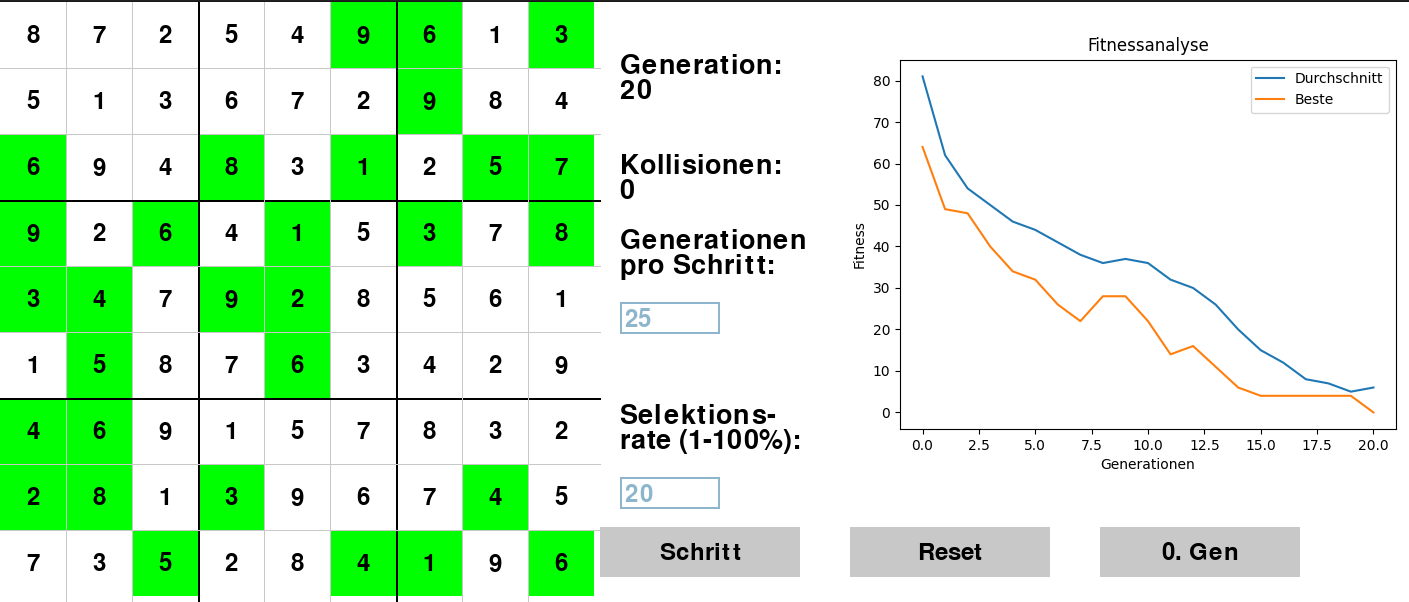
\includegraphics[width=\textwidth]{../../Pictures/GUI.png}

\noindent Das GUI nutzt die oben beschriebenen Methoden, um grafisch den Prozess der Lösung zu zeigen. 
Sie kann mit Debian über GUI.sh (GUI.sh) gestartet werden.
Vorraussetung ist Python. Die Module matplotlib und pygame werden über pip installiert.

\noindent Zunächst wird Populationsgröße und Sudokuauswahl abgefragt. 
Empfehlenswert sind Werte, die sich an der obigen Auswertung orientieren.
Die verschiedenen ungelösten Sudokus der Größe 9x9 in aufgearbeiteter Form können dabei in der Datei Sudokus (Sudokus.txt) gefunden werden (0 = leeres Feld).

\noindent Anschließend wird das Sudoku angezeigt. Dabei werden ursprünglich gegebene Felder grün und Felder mit Kollisionen rot markiert. 
Es werden auch die Anzahl an Generationen und die Gesamtzahl an Kollisionen im besten Sudoku dieser Generation gezeigt. Weiterhin werden in einem Graph die Best- und Durchschnittswerte der Generationen angezeigt.

\noindent Über den Parameter Schrittweite kann eingestellt werden, wie viele Generationen pro Schritt berechnet werden sollen. 
Mit dem Button "Schritt" wird dann die entsprechende Anzahl an Generationen berechnet und das beste Individuum, sowie der Verlauf der Fitness angezeigt. Dabei kann es bei höheren Generationszahlen (>500) durchaus zu längeren Wartezeiten kommen.
\newpage
\noindent In der Simulation werden dabei die oben empirisch ermittelten Bestwerte, also diagonales Crossover und die triviale Selektion verwendet. Die Selektionsrate kann zwischen jedem Schritt angepasst werden.

\noindent Ein zwingendes Abbruchkriterium ist nicht definiert. Vielmehr kann der Nutzer anhand der angezeigten durchschnittlichen Fitness der jeweiligen Generationen selbst entscheiden.

\noindentÜber "Reset" kann zum Startbildschirm zurückgekehrt werden.
"0. Gen" setzt die Simulation mit gleicher Populationsgröße und gleichem Sudoku zurück und schafft eine neue Startpopulation.
